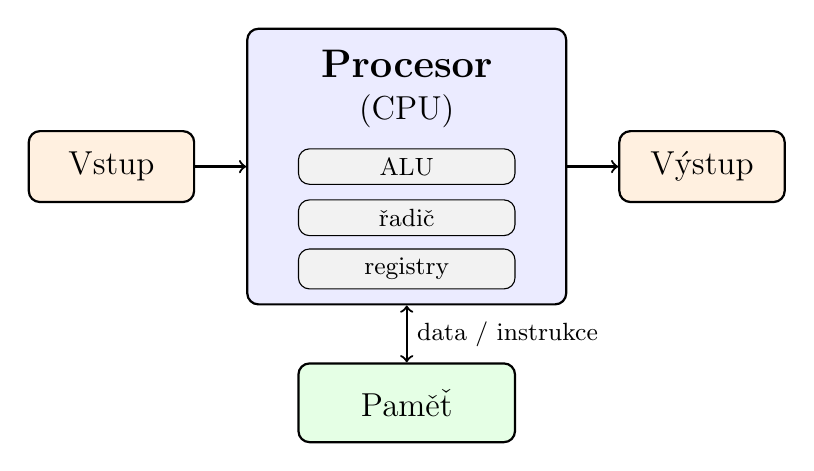
\begin{tikzpicture}[
    x=1cm, y=1cm,
    every node/.style={font=\small},
    unit/.style={
        draw,
        thick,
        rounded corners,
        align=center,
        minimum width=2.15cm,
        minimum height=0.75cm
    },
    subunit/.style={
        draw,
        rounded corners,
        align=center,
        fill=black!5,
        minimum width=2.75cm,
        minimum height=0.45cm,
        font=\small
    },
    arr/.style={->, thick},
    barr/.style={<->, thick}
]

    % CPU
    \node[
        unit,
        fill=blue!8,
        minimum width=4.05cm,
        minimum height=3.50cm
    ] (cpu) at (0,0) {};

    \node[font=\Large\bfseries] at (0,1.30) {Procesor};
    \node[font=\large] at (0,0.70) {(CPU)};

    \node[subunit] at (0,0) {ALU};
    \node[subunit] at (0,-0.65) {řadič};
    \node[subunit] at (0,-1.30) {registry};

    % Memory
    \node[
        unit,
        fill=green!10,
        minimum width=2.75cm,
        minimum height=1.00cm,
        font=\large
    ] (mem) at (0,-3.00) {Paměť};

    % I/O
    \node[
        unit,
        fill=orange!12,
        minimum width=2.10cm,
        minimum height=0.90cm,
        font=\large
    ] (inputnode) at (-3.75,0) {Vstup};

    \node[
        unit,
        fill=orange!12,
        minimum width=2.10cm,
        minimum height=0.90cm,
        font=\large
    ] (outputnode) at (3.75,0) {Výstup};

    % Arrows
    \draw[arr] (inputnode.east) -- (cpu.west);
    \draw[arr] (cpu.east) -- (outputnode.west);

    \draw[barr] (cpu.south) -- node[right, font=\small] {
        data / instrukce
    } (mem.north);

\end{tikzpicture}
